\chapter{Cargo Routing at Microtubule Intersections}

The following is adapted from a manuscript submitted to Proceedings of the National Academy of Sciences of the USA, currently under revision. The project was initiated by Michael Vershinin and Jared Bergman. Cargo navigation experiments were performed by Jared Bergman. Manasa Gudheti performed super-resolution microscopy. The model was created by Matt Bovyn and Jun Allard. Matt Bovyn wrote and performed simulations. The model was modified and developed to fit the experimental situation by Matt Bovyn with advice from Jun Allard, Steve Gross, Jared Bergman and Michael Vershinin. Jared Bergman, Matt Bovyn and Michael Vershinin wrote the main text. Matt Bovyn wrote the supplementary material, included here as appendix \ref{sec:model}.

\section{Introduction}

The microtubule (MT) network in eukaryotic cells is typically a dense, highly variable, three-dimensional (3D) mesh (Fig. \ref{fig:1}A). MT network topologies are known to vary widely between cells \cite{Schnorrenberg2016} and even between cells of the same type and lineage \cite{Dong2015}. Within a given network, MTs converge to form crossings at a variety of filament separations, and angles of intersection \cite{Huang2008}. Often, the crossings feature inter-filament separations that are comparable to the scale of the cargos found within the cell (Fig. \ref{fig:1}A). At these ``intersections," a cargo, with multiple motors on its surface, can potentially interact with several MTs simultaneously; a scenario known as Tug-of-War (ToW) \cite{Muller2008,Osunbayo2015}. The cargo can then either pass along the original MT, switch to the intersecting filament, pause, or detach. The probabilities of these outcomes are known to be sensitive to the 3D layout of the filaments \cite{Balint2013,Ross2008,Erickson2013} but the mechanistic details of this phenomenon are unclear. Given that the architecture/topology of the MT cytoskeleton serves as a persistent and pervasive backdrop for cargo transport \cite{Verdeny-Vilanova2017}, its role in cargo routing warrants a thorough investigation.

\begin{figure}
\floatbox[{\capbeside\thisfloatsetup{capbesideposition={right,top}}}]{figure}[\FBwidth]
{\caption[3D MT crossings and cargo navigational outcomes]{3D MT crossings and cargo navigational outcomes.\\
\textbf{(A)} 3D STORM image of MT cytoskeleton from BSC-1 cell. Color coding indicates relative depth. Scale bar: \SI{4}{\micro\meter}. (Inset) Perspective image of the MT crossing highlighted in dashed box. MT position fits (light blue and orange) are shown along with the registered photon originations (red and blue). MT separation at point of closest approach (double arrow) and MT-MT angle (protractor, dashed lines) are annotated for clarity. A few photon originations near MT-MT intersections are not shown for clarity of annotation.\\
\textbf{(B)} Illustration of in vitro 3D MT crossing with an MC undergoing ToW. BHs (large spheres) are permanently bound to MTs (blue and red). BHs are held in 3D via HOTs (light pink cones). MT plus ends are indicated (+ signs). For clarity, we only depict two motors on the MC (small bead), engaged on either MT. Navigational choices are indicated with arrows.\\
\textbf{(C)} Table showing switching probabilities as a function of 3D MT arrangement. Higher switch rates are highlighted by darker background. Significant differences (p $<$ 0.05, Barnard's test) are indicated by links.}\label{fig:1}}
{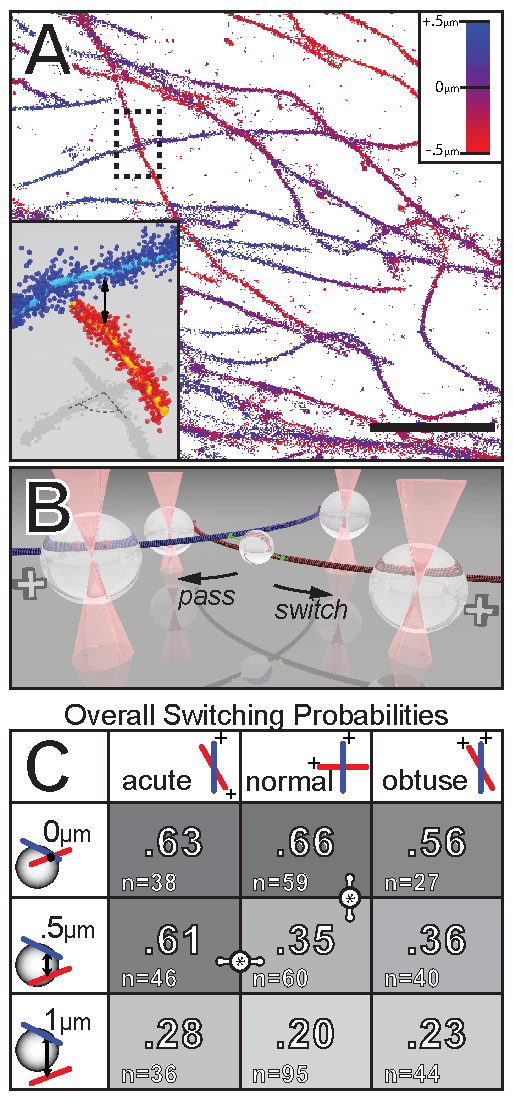
\includegraphics{project1/Fig_1FINAL}}
\end{figure}

The importance of MT cytoskeletal architecture is underscored by the fact that MT network remodeling occurs often in various diseases and during normal cellular processes. For example, neuritic de-arborization or restructuring is often encountered in neurodegenerative diseases \cite{VanBattum2015,DiPolo2015}. Microtubule remodeling is also observed in many neoplasias \cite{Parker2014} and is associated with pathways often disturbed in cancers \cite{Galmarini2003}. There is also evidence that suggests the geometry of the MT network, itself, acts as a regulator to tune insulin granule secretion in mouse pancreatic  $\beta$-cells \cite{Zhu2015}.
 
The cell can use multiple mechanisms to modulate its MT architecture. MTs can be locked in parallel \cite{Fink2009} or antiparallel \cite{Subramanian2010} alignment via cross-linking. Axonal branching generally shows a preference for normal angles \cite{Kalil2013}; low branch angles can arise from MT nucleating factors \cite{Petry2013}. The cell can set overall MT spacing by simply controlling the amount of polymerized tubulin, either via regulation of expression levels \cite{Dumontet1996} or filament stability \cite{Desai1997}. Filament spacing can also be controlled via MAPs that cross-link microtubules \cite{Hirokawa1988}. Microtubule and actin networks are often coupled and remodeling of one can drive structural changes in the other \cite{Chesarone2010,Young2008}. External factors which affect cell shape can also regulate MT network topology \cite{Gomez2016}. Finally, MT crossings are known to be special loci for intracellular regulation \cite{Hamant2013}. Currently, the implications of these topology variations for cargo logistics and overall biomechanics are not quantitatively understood.
 
Decoupling the influence of the MT network's 3D topology from regulatory protein factors is challenging. The same pathways that drive network remodeling can also couple to motor regulation. The result is that, to date, the impact of geometric changes in MT networks on intracellular cargo transport has been difficult to isolate and quantitate. It is common in biology to think in terms of chemical regulation. However, to truly understand how intracellular cargo transport functions, it is critical to gain a baseline understanding of how the 3D MT geometry alone impacts cargo distribution, starting at the most fundamental level of the MT network: individual MT-MT intersections.
Studying cargo navigational behavior as a function of 3D network geometry poses considerable experimental challenges. In vivo investigations cannot easily decouple chemical and topological regulation, as discussed above. Moreover, although theoretical work highlights its importance \cite{Erickson2013}, in vitro bead assays that use traditional MT-glass deposition techniques are also unable to model MT-MT crossings with controlled filament separation \cite{Ross2008,Vershinin2007}.
 
To address this question, we developed an in vitro system to suspend and dynamically manipulate multiple individual MT filaments in 3D. Each MT is manipulated individually via holographic optical trapping (HOT) of two or more bead handles (BH), as previously described \cite{Bergman2015}. We used this bottom-up approach to systematically construct MT-MT intersections featuring various angles and separations. We then measured the statistics of kinesin-1 driven model cargo (MC) transport on these model MT geometries, and used this data to constrain 3D simulations. We show from experimental data and theoretical analysis that navigational outcomes exhibit systematic variation based on 3D MT intersection geometry. Further, we propose dynamic mechanisms that explain the observed preferences.

\section{Results}

\subsection{Experimental Setup}

The broad aim of this work is to understand the impact of cytoskeletal geometry on intracellular transport. A comprehensive experimental model of all possible geometries (e.g. Fig \ref{fig:1}A) is well beyond the scope of any singular study, so we restricted our scope to representative model scenarios. We focused on the simplest type of intracellular MT intersections where just two filaments cross (Fig. \ref{fig:1}A, inset). We used silica microspheres, driven by full length KHC homodimers, as our MC. This is a common, albeit simplified, model for in vitro work. We chose to focus on assays outside the single-molecule regime because there is substantial evidence that
cargos in cells are often driven by multiple motor ensembles, and indeed multiple-motor ensembles are essential for a ToW to develop.

We used in vitro 3D MT manipulation via HOT \cite{Bergman2015} to examine three filament spacings: zero, radius, and diameter of the MC. Our MCs were \SI{1}{\micro\meter} in diameter, hence we constructed and observed MC transport across model intersections featuring 3 separation distances (\SI{0}{\micro\meter}, \SI{.5}{\micro\meter}, and \SI{1}{\micro\meter}). We decided to only parametrize this geometric range because the probability of a cargo interacting with both MTs for crossing separations greater than the cargo diameter quickly becomes negligible. For each separation distance, we examined three different angles of intersection, acute (MT polarities nearly counter aligned), normal (\SI{90}{\degree}), obtuse (MT polarities nearly aligned), for a total of nine geometric conditions.

We chose silica microspheres as our MCs because their density is 2.2x that of water. This biased the cargo to hang below the MT to which it was engaged, although Brownian motion along all three axes was both expected and observed. Thus, in our setup, we always deposited the MC (via HOT) onto the ``overpass" MT, such that the hanging cargo would be likely to encounter the lower, crossing MT (Fig. 1B). With this setup, our \SI{0}{\micro\meter} separation experiments resemble the ``underpass" MT geometry in prior crossing experiments, in which MTs were attached to a glass substrate \cite{Ross2008,Vershinin2007}. However, our experimental model allows for MT bending, twisting, and vibrations which cannot be recapitulated when MTs are firmly attached to a solid substrate. The absence of the solid glass substrate in our work is a major difference since the cargo can explore many more three-dimensional paths as it negotiates the intersection.

\subsection{Final navigational outcomes depend on 3D geometry}

For each of the nine MT network arrangements in our assays, we quantified final cargo routing outcomes strictly in terms of, ``switching" or ``passing", because detachment at intersections was negligible. In addition, we do not report pause events, because we can characterize the entire navigational event, even in cases where the MC navigational choice takes several seconds to make. Below, we report switching probability only, as passing probability is complementary.

Our results suggest that 3D MT network topology alone can be an effective regulator of cargo routing (Fig. \ref{fig:1}C). Geometries in the upper left corner of the table promote switching while those in the lower right corner promote passing. Therefore, routing outcomes are determined by multiple geometric factors interacting in non-trivial ways. Disentangling these factors by intuition alone is challenging, therefore we relied upon \textit{in silico} modeling. Helpfully, many fine mechanistic details are resolved by our experimental approach (see below), which constrain the \textit{in silico} model.

\subsection{Characterization of Tug-of-War events}

A cargo that does not engage in a ToW, does not switch; hence precisely distinguishing between ToW and non-ToW events is critical to dissect the mechanisms that lead to differential switching probabilities. Our spatiotemporal resolution is sufficient not only to establish whether a ToW took place, but also to precisely determine ToW durations.

We can readily identify ToW start and end by observing significant MC displacements away from MT axes and associated MT deflections (Fig. \ref{fig:2}A). MC tracks for representative pass (Fig. \ref{fig:2}B), and switch (Fig. \ref{fig:2}C) events are shown, along with their displacements projected along the axes of the intersecting MTs. A ToW start can be identified with the beginning of a sustained displacement upon the crossing MT's axis. ToW end can then be identified when the cargo snaps back upon dissociation from either the primary or crossing MT. BH displacements can also be used as an indicator of a ToW because the MC motors engaged in a ToW will exert force on the MTs that ultimately displaces the BHs (Fig. \ref{fig:1}B, \ref{fig:2}A \textit{middle}, D).

\begin{figure}
\centering
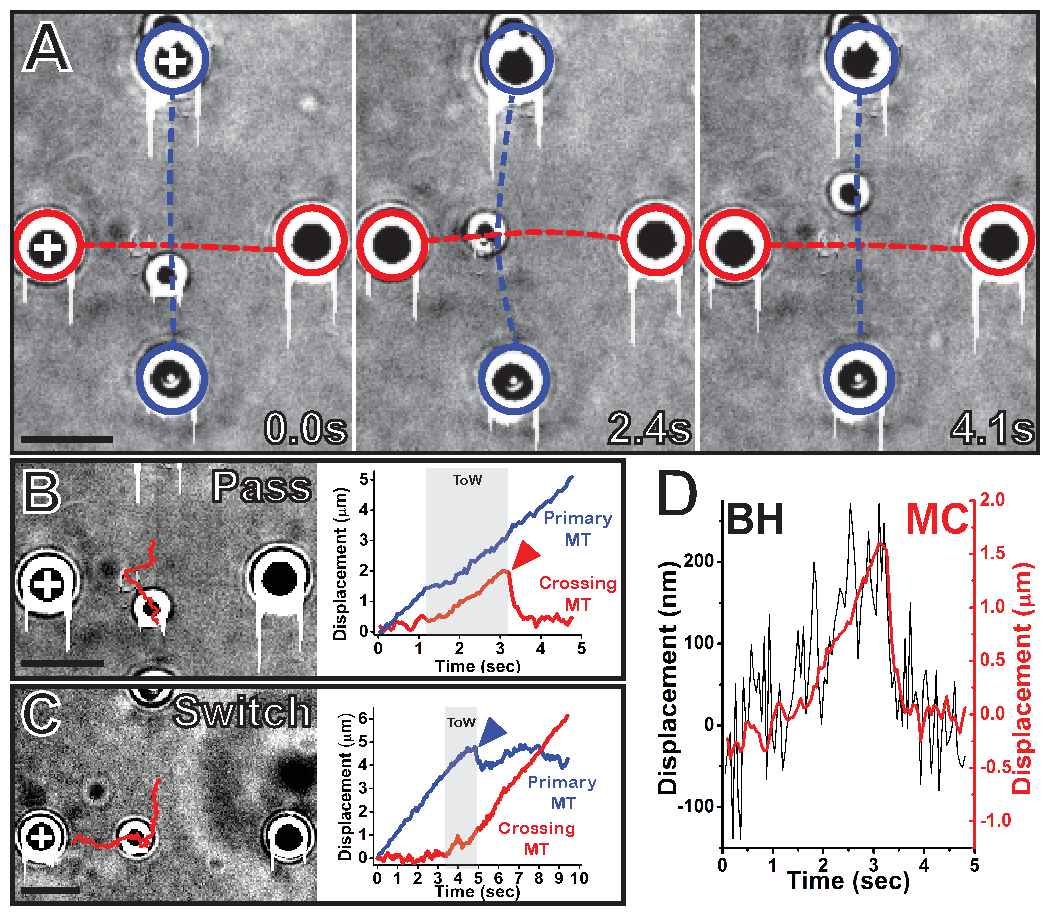
\includegraphics[scale=.7]{project1/Fig_2FINAL}
\caption[Identification and quantification of ToW]{Identification and quantification of ToW. \\
\textbf{(A)} Three video frames: before, during, and after ToW (left to right). Circles show BH
positions in the left panel and are positioned identically in middle and right panels. Dashed lines highlight positions of MTs inferred from video for each frame. Blue and red color scheme represents over- and underlying components respectively (\SI{.5}{\micro\meter} separation). Displacement of the top BH relative to its fiducial circle indicates presence of ToW (middle panel); its original position is restored once ToW has ended (right panel). White plus signs indicate the MT plus ends. Frame timings shown in lower right corner. \\
\textbf{(B)} Analysis of the pass event shown in panel (A). Left panel: Trajectory of MC (red) overlaid on one cropped video frame. Right panel: MC displacements projected along the primary (blue) and crossing (red) MT directions. Red arrowhead highlights the snapback event which is typical of a ToW conclusion. Gray band: ToW temporal extent ($\sim$ 1.9 s). \\
\textbf{(C)} Analysis of a switch event. Left panel: Trajectory of MC (red) overlaid on one video frame. Right panel: MC displacement projected along the primary (blue) and crossing (red) MT's axes (\SI{.5}{\micro\meter} separation). Blue arrowhead highlights when the MC undergoes a ``snapback", an event which is typical of a ToW conclusion. Gray band: ToW temporal extent ($\sim$ 1.6 s). \\
\textbf{(D)} MC displacement along the crossing (red) MT axis shown in (B) overlaid onto trace of BH displacement from trap center, due to ToW (for the top BH in (A)). All scale bars are \SI{5}{\micro\meter}.}
\label{fig:2}
\end{figure}

Although BH displacements can help confirm ToW presence and duration, their greatest benefit is that they are an indicator of how many motors were exerting force on the bead. We set the trap stiffness at $\sim$\SI{1}{\pico\newton}/\SI{100}{\nano\meter}, so that a single kinesin motor could not pull the BH out of the trap (escape event) but two or more motors working together could do so readily (Fig. \ref{fig:BHforce}). Quantifying collective activity of multiple motors via trap escape forces is a well-established approach both in vivo \cite{Ashkin1990,Gross2002} and in vitro \cite{McKenney2010} and has been validated in silico \cite{McKenney2010}. This setup allowed us to control the surface density of motors on MCs by discarding assays in which BH escape fraction exceeded 25\% of total events. This provided refined control on top of the more crude and variable approach of controlling motor concentration at incubation time. It also provided confidence that ToWs in our assays were dominated by forces from 1-2 kinesin motors; more motors are likely engaged on the MT but not all are positioned to exert force during the ToW.

\subsection{Mechanisms of cargo routing}

The ability to sensitively detect ToW events allowed us to quantify their probability. We could then also examine the probability for the cargo to pass or switch, conditional on ToW occurrence. This analysis is informative because these probabilities reveal different aspects of cargo dynamics (Fig. \ref{fig:3}). Our data indicates that ToW probability is sensitive to 3D geometry: it is higher for narrower filament separations, and for acute/obtuse angles (Fig. \ref{fig:3}A). For \SI{0}{\micro\meter} separations, ToW probability is so high that significant differences as a function of angle may not be practical to measure. A different pattern of navigational outcomes emerges when trivial passes (no-ToW events) are omitted (Fig. \ref{fig:3}B vs Fig. \ref{fig:1}C). Four out of nine geometries show switch probabilities close to 50\%. We also record switch probabilities that are significantly higher than 50\% for the following geometries: \SI{0}{\micro\meter} normal, \SI{0}{\micro\meter} acute, and \SI{.5}{\micro\meter} acute (p $<$ .05 Barnard's test). We conclude that geometric constraints can promote or inhibit switching outcomes for ToW events.

\begin{figure}
\floatbox[{\capbeside\thisfloatsetup{capbesideposition={right,top}}}]{figure}[\FBwidth]
{\caption[Cargo navigation flow chart, with associated outcome probabilities]{Cargo navigation flow chart, with associated outcome probabilities. \\
\textbf{(A)} Probabilities of ToW, as a function of 3D MT network geometry. \\
\textbf{(B)} Probabilities of switching conditional on ToW taking place, as a function of 3D MT network geometry. ** indicate probability is significantly higher than 50\% (p$<$0.05, Barnard's test).} \label{fig:3}}
{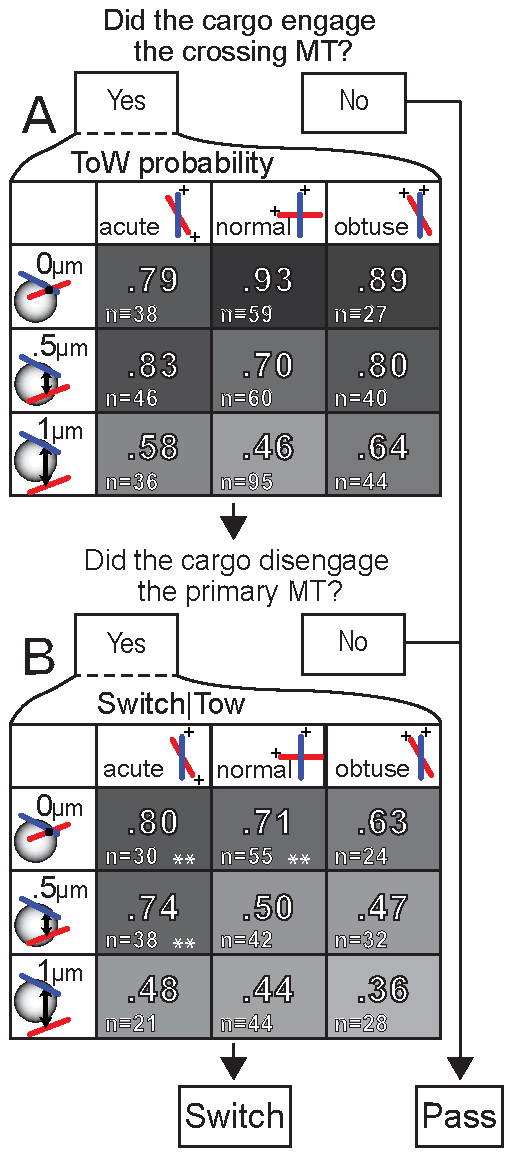
\includegraphics{project1/Fig_3FINAL}}
\end{figure}

\subsection{A mathematical model of cargo transport reproduces observed switch probabilities}

As mentioned above, it is difficult to disentangle the mechanism through which each factor acts to (in concert) determine ToW and switching probabilities. Therefore, to gain further insight into the mechanism determining cargo routing, we constructed an \textit{in silico} model of cargo transport. This model allows us to examine experimentally unobservable details, such as how motor locations, bound states and force states change with time.

The model incorporates relevant experimental details including: the well-established properties of kinesin-1 motors, and cargo translational and rotational diffusion, however, simulated MTs do not move, twist, or bend (Fig. \ref{fig:4}A). 500 cargo trajectories were simulated independently for each assay geometry, and probabilities of ToW and switching were then determined analogously to the experimental data. For full simulation details and parameter fitting procedure, see \ref{description} and \ref{sec:simulation}. Briefly, there were two parameters that could not be established from current experiments or prior literature: average motor number attached to MCs and each motor's on-rate. These two parameters were constrained by matching three experimental observations: ToW probability as a function of geometry (Fig. \ref{fig:ToW_fit}), fraction of BH escape events and MC run lengths (Fig. \ref{fig:run_length_fit}). Thus, the model is fully constrained and therefore predictive.

We found good agreement between experimentally observed and theoretically predicted probabilities of ToW'ing and switching (Fig. \ref{fig:4}B-D). We now turn to investigation of the quantitative details of ToW and switching (next two sections), and their implications for the mechanisms of cargo navigation at MT intersections.

\begin{figure}
\centering
\includegraphics{project1/Fig_4FINAL}
\caption[Mathematical model of navigational outcomes]{Mathematical model of navigational outcomes. \\
\textbf{(A)} Snapshots of simulated cargo activity at an intersection (color coding as in Fig. \ref{fig:3}).
Examples of Pre-ToW, ToW, and post-TOW states are shown (left, middle, right respectively). Motors bound to the primary MT are shown in cyan. Motors bound to the crossing MT are shown in magenta. Unbound motors are shown as green spherical protrusions from MC; sphere radius represents motor's maximal reach. Bead's ``prime meridian" demarcated to emphasize rotational movement.
\textbf{(B)} Simulated probabilities to engage in ToW. Probability of undergoing ToW for each geometry is shown as thin symbols (error bars: SEM). Experimental data is shown as large symbols (error bars: 95\% C.I.). Experimental data points for \SI{.5}{\micro\meter} geometries shifted slightly horizontally to aid the eye.
\textbf{(C)} Simulated probability to switch, given the cargo engaged in ToW. Simulated and experimental data represented as in (B).
\textbf{(D)} Simulated probability to switch, overall, i.e. the product of probability to ToW (B), and probability to switch, given ToW (C). Simulated and experimental data represented as in (B).
\textbf{(E)} Snapshot of a ToW for \SI{0}{\micro\meter}, \SI{90}{\degree} geometry. Here, primary MT motors are blocked from passing the intersection by the crossing MT at \SI{0}{\micro\meter}. Bound and unbound motors represented as in (A).
\textbf{(F)} Probability to switch increases with increasing simulated fluid viscosity. Error bars: SEM.
\textbf{(G)} Force exerted by crossing MT on the cargo for \SI{.5}{\micro\meter} geometries (mean $\pm$ SEM).}
\label{fig:4}
\end{figure}

\subsection{The influence of intersection geometry on ToW probability}

The longer a cargo spends within reach of the primary and intersecting MTs (henceforth, the ToW zone), the more chances unbound motors on the cargo have, to engage the intersecting MT. This phenomenon can be understood from a simple, heuristic model. If we consider the cargo as having a single rate of binding to the crossing MT given by $k_{\text{on}}^\text{macro}$, the probability the cargo binds to the crossing MT before leaving the ToW zone is given by 
\begin{equation} \label{eq:rate_war}
p(\text{ToW})=\frac{k_{\text{on}}^\text{macro}}{k_{\text{on}}^\text{macro} +  v / d_\text{ToW} },
\end{equation}
where $v$ is the cargo velocity and $d_\text{ToW}$ is the length of the ToW zone. This simple model can accurately reproduce experimental ToW probabilities for both the \SI{.5}{\micro\meter} and \SI{1}{\micro\meter} separation distance geometries (Fig. \ref{fig:heuristicEXP}), but not for the \SI{0}{\micro\meter} separation geometries. This strongly suggests that there are mechanisms at play for \SI{0}{\micro\meter} separations which are not present at other distances (see below).

On the other hand, our full model closely recapitulates all experimental ToW probabilities, including \SI{0}{\micro\meter} separation data. It is encouraging that the model captures several \textit{a priori} intuitive features of the system. For \SI{0}{\micro\meter} geometries, if a cargo is driven by multiple motors then there is guaranteed to be a pool of motors able to bind the crossing MT (namely, the already engaged motors). Thus, we \textit{a priori} expect the ToW probability for all angles to be close to 1, which our model reproduces. For \SI{.5}{\micro\meter} and \SI{1}{\micro\meter} geometries, we expect higher ToW probability for longer ToW zones (acute and obtuse angles). Indeed, simulated ToW probabilities were smallest for \SI{90}{\degree} intersections (Fig. \ref{fig:4}B). Also, as expected, they were symmetric about the normal angle (since kinesin binding is not affected by MT polarity). Simulated ToW probabilities also increased when MT separation decreased from \SI{1}{\micro\meter} to \SI{.5}{\micro\meter}, as expected. When the intersecting MT encounters the MC's midsection, at \SI{.5}{\micro\meter} separations, it samples more of the bead's surface area (especially when rotational diffusion is taken into account). Hence, at \SI{.5}{\micro\meter} separation, more motors are given a chance to engage on the crossing MT, which increases ToW probability.

\subsection{The influence of intersection geometry on navigational outcomes, given ToW}

Experimentally, we observe a large range of geometries (most \SI{.5}{\micro\meter} and \SI{1}{\micro\meter} geometries) where the conditional probability to switch is $\sim$50\%. At first glance, this appears to be a relatively intuitive result: if ToW lasts $\sim$\SI{1}{\second} or more (our experimental ToW durations average $\sim$\SI{3}{\second}, Fig. \ref{fig:ToWtimes}), then the motor team engaged on the crossing MT should be able to reach steady state \cite{Erickson2011}, and become equal in number to the primary motor team. With two equivalent ways to proceed, the probability of either choice would indeed be $\sim$50\%. However, such a consideration is too simplistic as we discuss below.

Experimental results allow for sensitive identification of ToW, so that ToW events can be analyzed separately from trivial ``no-ToW" intersection passages (Fig. \ref{fig:3}). The same analysis can be performed for simulated events (Fig. \ref{fig:4}B-D). A careful analysis of the simulations helps us shed light on the mechanistic details of cargo navigation.

We first assessed whether the number of motors in the two ensembles is in fact equal in our simulations. We find that contrary to na\"ive expectation, the number of engaged motors on the secondary MT is comparable but consistently lower than that on the primary MT (ratio of $\sim$0.7; Fig. \ref{fig:num_engagedEXP}). The reason is that the motors already engaged on the primary MT constrain the bead from full range of linear and rotational diffusion. Once a ToW starts, the bead diffusion is even more constrained; this curtails the number of motors that can reach the secondary MT. Thus, the team of motors pulling along the primary MT generally has an advantage. However, the two paths to proceed are not equivalent either. The crossing MT itself can serve as an obstacle for bead progress and exert a force which hinders the MC from passing (Fig. \ref{fig:4}G). The smooth decrease from passing to switching prevalence across our experimental geometries (Fig. \ref{fig:3}B) therefore reflects the balance between net motor activity (which is biased in favor of moving along the primary MT) and steric hindrance from the crossing MT.

\subsection{The limits of geometric regulation}

Our results establish that a single MT intersection can significantly bias cargo routing towards more switching or more passing. Can a single MT intersection produce a near 100\% bias for switching or passing? What are the mechanisms which affect these limits? It is easy to see that $\sim$100\% passing naturally occurs for intersections with filament separation much greater than MC diameter. Is 100\% switching attainable? To address this, we consider two special cases which lead to elevated probability to switch, and their broader implications for geometric regulation. For completeness, we also discuss each experimental geometry individually in \ref{sec:results}.

\subsection{Low filament separations}

A closer look at the geometric setup (Fig. \ref{fig:4}E) makes it clear that the \SI{0}{\micro\meter} case is qualitatively distinct. At \SI{0}{\micro\meter} separation, the crossing MT sterically hinders the motors engaged on the primary MT, but not for the MC itself. To pass, the cargo can ``hurdle" over the crossing MT due to Brownian motion but this is improbable for our large silica MCs (density $\approx$ 2.2x water). Hurdling would also be unlikely in the viscous cytosolic environment (even for smaller cargos). The only other way to pass is by a mechanism we refer to as ``monkey-barring." To pass via monkey-barring, the MC must first diffuse underneath the crossing MT so that some of the unengaged motors on its surface could bind to the distal side of the primary MT (Fig. \ref{fig:5}A). The motors proximal to the crossing MT must then gradually disengage. The above suggests that passing at \SI{0}{\micro\meter} separation should have a sensitive dependence on the diffusion properties of the medium. This is indeed seen in our simulations (Fig. \ref{fig:4}F). In fact, for viscosities close to intracellular range, where cargo diffusion is suppressed, the preference to switch approaches 100\%.

\begin{figure}
\centering
\includegraphics{project1/Fig_5FINAL}
\caption[Mechanisms that elevate switch probabilities]{Mechanisms that elevate switch probabilities.\\
\textbf{(A)} Illustration of MC approaching a normal intersection with a separation of \SI{0}{\micro\meter}. 1) Motors engaged on the primary MT can detach, then rebind to the crossing MT. 2) Unengaged motors can bind the crossing MT. 3) Unengaged motors can bind the primary MT at a site distal to filament intersection - the first step in the monkey-barring mechanism. All motors are in green regardless of engagement status.\\
\textbf{(B)} Illustration of MC engaged in ToW at an acute \SI{.5}{\micro\meter} intersection. A minimal ToW with only two motors is shown for visual clarity. The forces exerted by motors are counter aligned (grey arrows) and serve to wedge the MC between the MTs. Red arrows point to MT plus ends.}
\label{fig:5}
\end{figure}

\subsection{Acute angles / intermediate separations}

Why is switching more prevalent for \SI{.5}{\micro\meter} acute geometry? Again, this must be due to the crossing MT acting as a strong hindrance, but the mechanism cannot be the same as in the previous section. Here, monkey-barring is not feasible but hurdling is. Evidently, in this case, for switching probability to be elevated, hurdling must be suppressed. The vertical forces associated with the ToW for \SI{.5}{\micro\meter} acute geometry pull the MC between MTs. This effectively wedges the cargo between the two MTs, which indeed prevents hurdling. We refer to this mode of steric hindrance as ``chop-sticking" (Fig. \ref{fig:5}B). Note that in our simulations, MTs were not allowed to bend, which would likely be a factor under experimental conditions. In reality, the two motor teams engaged in a ToW during chop-sticking would be expected to pull the two MTs closer together, which would make the crossing MT an even stronger obstacle to passing. This is likely the reason why experimentally observed switching probability for \SI{.5}{\micro\meter} acute geometry is somewhat higher than theoretical prediction.

\section{Discussion}

Cargos driven by multiple motors can exhibit incredibly complex behavior. Even when one considers this for a single cargo moving along a single MT, the system complexity is sufficient to lead to highly non-trivial emergent behaviors \cite{Kunwar2008,Jamison2010}. The number of motors in biologically relevant systems is typically small which necessitates highly detailed experiments and modeling to account for not only averaged behavior but also the effect of fluctuations. The addition of just one more filament adds such complexity that the emergent behaviors can dramatically diverge to give rise to discrete outcomes: passing and switching. It is therefore a fascinating model system to study emergent behaviors in biology.

We have modeled this problem in a highly controlled experimental environment in which we imposed very specific restrictions on cargo size and other experimental variables. We then performed highly detailed modeling of our system \textit{in silico} to generalize our experimental results. We were thus able to infer the key processes which underlie our observations. This enables us to extrapolate how cargo routing might function in cells (and other environments).

Our analysis shows that the team of motors driving the cargo along the primary MT is generally at an advantage, even when the ToW is prolonged. This implies that there is an inherent bias to pass. However, our data shows that for many geometric conditions passing and switching is balanced, and in some cases, switching dominates. The missing factor which shifts the balance between passing and switching is the extent to which the crossing MT acts to sterically hinder the motors progressing along the primary MT.

We show that the crossing MT can indeed be an effective obstacle, especially when it intersects at an acute angle with intermediate separation, or near-zero separation. Both types of geometries significantly inhibit passing but via different mechanisms: intermediate separations with acute angles lead to chop-sticking, while near-zero filament separations mean that passing is only accessible by means of monkey-barring (which is an unlikely event). These results imply that the cell could selectively route cargos of different sizes by controlling MT intersection angle and spacing.
Our simulations closely follow the experimental results but two important deviations are seen: the conditional probability to switch given that ToW already started is higher in experiments than in simulations. Also, the time a cargo spends at the intersection is higher in the experiment than in simulation (Fig. \ref{fig:ToWtimes}). In both cases, the discrepancy is clearly linked to the fact that we model MTs as an infinitely rigid rod. To date, MT rigidity has been mostly studied separately from MT-based transport. Our work suggests that MT bending and more generally biomechanics of the MT cytoskeleton must be taken into account in future studies of intracellular motility as they are a non-negligible contributor to cargo routing.
                      
A faithful and detailed \textit{in silico} model of cargo motility and the ToW process enables us to then speculate about cargo navigation patterns beyond our specific conditions. First, we show that if viscosity increases, then switching would be further favored for near-zero filament separations. In effect, our simulations lead us to speculate that not only MT geometry but also local microrheology can be a regulator of cargo routing.

We also predict that extremely short motors should find reaching across the crossing MT for near-zero separations particularly difficult, so cargos driven by very short motors would preferentially switch at intersections. It is tempting to speculate that overall kinesin length evolved to reduce the probability of cargos getting trapped in filament-filament switching loops.

On a more architectural level, our results suggest that for each cargo type and size there is a critical MT density at which efficient transport can be inhibited by too much switching at intersections. This prediction from the single molecule level dove-tails with the more qualitative observations for the insulin secretion process \cite{Zhu2015}.

Our work opens many new directions for future work, including studies of more complex intersections, more complex cargos and motor complexes. Together these baseline studies can then serve as a basis for studying chemical regulation of motility in the context of cytoskeletal network geometry. A gradual from-the-bottom-up increase in complexity can then gradually lead to comprehensive quantitative understanding of intracellular cargo fluxes, from a single-molecule mechanistic perspective.

\section{Materials and Methods:}

\subsection{Optical trapping and 3D motility experiments:}

Our holographic optical trapping and bead assays were performed as previously described \cite{Bergman2015}. However, in present work, enzymatically dead KIF5A heavy chain dimers were adsorbed onto bead handles non-specifically. Switch/pass outcomes were assessed live during the experiments from the video feed and recordings were conducted until definitive outcome was attained. Video records of bead positions were tracked using custom software (MATLAB, MathWorks, Natick, MA).

\subsection{Super-resolution imaging:}

African green monkey kidney epithelial (BSC1) cells were labeled with primary antibody, alpha-tubulin, against microtubules followed by secondary antibody labeling with Alexa Fluor 647. Super-resolution images were recorded with a Vutara commercial microscope (Bruker, Salt Lake City, UT) based on the single molecule localization (SML) biplane FPALM technology \cite{Juette2008,Mlodzianoski2009}.

Microtubules were imaged using a 647 nm excitation laser, and 405 nm activation laser in photoswitching buffer comprising of 20 mM cysteamine, 1\% betamercaptoethanol, and oxygen scavengers (glucose oxidase and catalase) in 50mM Tris+10 mM NaCl+10\% glucose buffer at pH 8.0. Images were recorded using a 60x/1.2 NA Olympus water immersion objective and Photometrics Evolve 512 EMCCD camera with gain set at 50, frame rate at 50 Hz and maximal powers of 647 nm and 405 lasers set at 8 and 0.05 kW/cm$^2$ respectively.

Data was analyzed by the Vutara SRX software (version 6.00). Single molecules were identified by their brightness frame by frame after removing the background. Identified particles were then localized in three dimensions by fitting the raw data in a customizable region of interest (typically 12x12 pixels) centered around each particle in each plane with a 3D model function which was obtained from recorded bead data sets. Fit results were stored as data lists for further analysis.

\subsection{Statistical analysis:}

Much of our data is in the form of contingency tables. Barnard's exact tests were used to assess significance of differences between outcomes.

\subsection{Simulations:}

See Appendix \ref{sec:model}.

\section{Acknowledgements:}

We are grateful Dr. Erik Jorgensen for helpful discussions and guidance on super-resolution imaging of microtubules. This work was supported by NSF grant number ENG-1563280 to M.V., NIH T32 EB009418-07 to M.B. and NIH R01 GM123068 to J.A. and S.G.